% -----------------------------------------------
% Template for ISMIR Papers
% 2016 version, based on previous ISMIR templates

% Requirements :
% * 6+1 page length maximum
% * 2MB maximum file size
% * Copyright note must appear in the bottom left corner of first page
% (see conference website for additional details)
% -----------------------------------------------

\documentclass{article}
\usepackage{ismir,amsmath,cite}
\usepackage{graphicx}
\usepackage{color}

% Title.
% ------
\title{Modulo7 : A full stack Music Information Retrieval And Structured Querying Engine}

% Note: Please do NOT use \thanks or a \footnote in any of the author markup

% Single address
% To use with only one author or several with the same address
% ---------------
%\oneauthor
% {Names should be omitted for double-blind reviewing}
% {Affiliations should be omitted for double-blind reviewing}

% Two addresses
% --------------
%\twoauthors
%  {First author} {School \\ Department}
%  {Second author} {Company \\ Address}

%% To make customize author list in Creative Common license, uncomment and customize the next line
%  \def\authorname{First Author, Second Author} 


% Three addresses
% --------------
\threeauthors
  {First Author} {Affiliation1 \\ {\tt author@ismir.edu}}
  {Second Author} {\bf Retain these fake authors in\\\bf submission to preserve the formatting}
  {Third Author} {Affiliation3 \\ {\tt author3@ismir.edu}}

%% To make customize author list in Creative Common license, uncomment and customize the next line
%  \def\authorname{First Author, Second Author, Third Author} 

% Four or more addresses
% OR alternative format for large number of co-authors
% ------------
%\multauthor
%{First author$^1$ \hspace{1cm} Second author$^1$ \hspace{1cm} Third author$^2$} { \bfseries{Fourth author$^3$ \hspace{1cm} Fifth author$^2$ \hspace{1cm} Sixth author$^1$}\\
%  $^1$ Department of Computer Science, University , Country\\
%$^2$ International Laboratories, City, Country\\
%$^3$  Company, Address\\
%{\tt\small CorrespondenceAuthor@ismir.edu, PossibleOtherAuthor@ismir.edu}
%}
%\def\authorname{First author, Second author, Third author, Fourth author, Fifth author, Sixth author}


\sloppy % please retain sloppy command for improved formatting

\begin{document}

%
\maketitle
%
\begin{abstract}
This paper describes a novel Music Information Retrieval and Structured Querying framework named Modulo7. Modulo7 is a full stack implementation (both client and server side software) which facilitates indexing variegated sources of music (midi, mp3, music xml and digitized sheet music files). It implements a similarity search engine based on customized vector space representations of songs, an efficient indexing and persistent storage mechanism and an interface for querying attributes based on SQL(Structured Querying Language) like principles. This papers describes the design goals and implementation details of the framework and outlines the speed up and scale up results over input sources and other MIR frameworks and discusses potential improvements. \\\\
\textbf{Keywords : MIDI, Music XML, MP3, Music Retrieval, SQL}
\end{abstract}
%
\section{Introduction}\label{sec:introduction}

Given the explosive growth of Music Information Retrieval research, several approaches and software suits have been designed to tackle generic problems such as efficient indexing, similarity searches, archival methods, structured and un-structured querying,feature extraction, audio and digital signal processing etc. A vast majority of the MIR frameworks in academia tend to approach very specific problems and does not support scalability as a significant end goal in itself \cite{mirproblems}. Moreover, industry applications predominantly treat MIR applications based on collaborative filtering approaches \cite{amazonreco} and/or manual annotation \cite{musicgenomepandora} instead of structural analysis of music sources. However these frameworks scale very well to large datasets. \\\\
Modulo7 is an attempt to capture the best features of both worlds. Modulo7 converts different music sources (midi, musicxml files, sheet music png/jpeg files and mp3) into a single unified symbolic representation. It indexes songs on global properties (artist name, key signature, time signature etc) and provides a vector space implementation for similarity searches and querying based on the SIMILIE \cite{similie} platform and extended to include chords and polyphony. As a consequence, Modulo7 acts as an end to end software suite for Music Information Retrieval including client side querying, searching, indexing and persistent store mechanism. The broad goals of Modulo7 can be summarized as

\begin{enumerate}
\item To efficiently store and index variegated data formats into a unified format while keeping symbolic information intact.
\item To create a framework for music retrieval from multiple music formats and in effect facilitate comparing songs of different formats.
\item To query/search relevant songs based on a quantified version of music theoretic principles. 
\item To build a full stack open source platform for end to end MIR tasks. Modulo7 is hosted at \cite{m7code}
\end{enumerate}

%
\section{Relevant Work} \label{sec:relevantwork}

Music Information Retrieval is a vast and interdisciplinary body of work. In order to facilitate research in MIR, several software suites and frameworks have been developed in the academic community in the past. Notable amongst them are software suites like jMIR \cite{jMIR} for automatic feature extraction from audio and midi sources to be used as input into machine learning algorithms for genre classification, Marsyas \cite{marsyas}, essentia \cite{essentia} and librosa \cite{librosa} for audio processing, humdrum \cite{humdrum} for automated musicological research, gamera \cite{gamera} for optical music recognition and symbol identification and SIMILIE \cite{similie} for melodic similarity analysis. \\\\
On top of the effort done by there has been significant effort undertaken by companies in the field of MIR with an emphasis on music recommendation. For instance Amazon implements a collaborative filtering approach by quantifying a consumer's shopping behavior \cite{amazonreco}. Pandora on the other hand utilizes an approach in which trained musicologists manually classify similarity between artists and songs \cite{musicgenomepandora} which is subsequently consumed by Pandora's APIs for similarity searches. Shazam \cite{shazam} implements a database music fingerprints and supports music ID as a service. 
 
\section{Software Design}\label{sec:architecture}

This section details the software design of the Modulo7 most notably its architecture and a typical consumer work-flow description(i.e. how is Modulo7 initialized and consumed as a service). 

\subsection{Software Architecture and Design}

The Modulo7 architecture can be visualized in figure \ref{fig:architecture} and is broadly divided into the following components. 

\begin{figure}[h]
\begin{center}
{\framebox{
 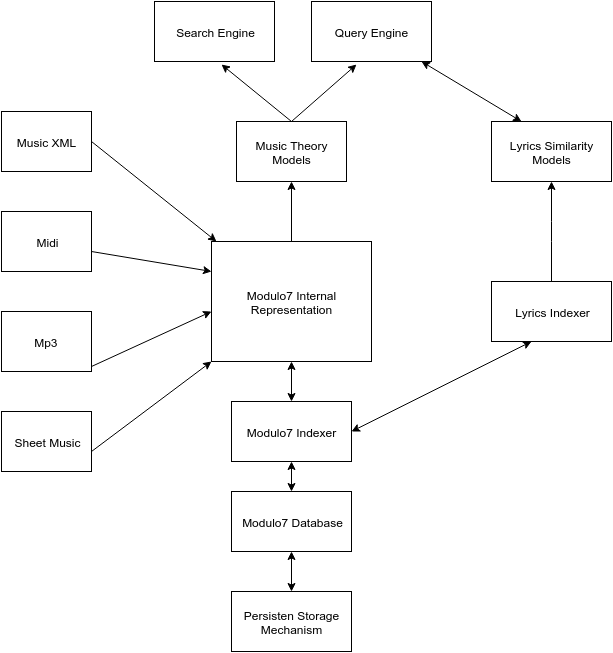
\includegraphics[width=\columnwidth]{Modulo7Architecture.png}}}
 \caption{A block diagram of the Modulo7 Architecture.}
 \label{fig:architecture}
\end{center}
\end{figure}

\begin{enumerate}
\item \textbf{Music Parsers: } Components that individually parse different music sources into a unified symbolic representation. as visualized in figure \ref{fig:document}. This object can be stored in memory or in a persistent serialized state via Apache Avro library. Depending on the source of the file, the parser utilizes a different approach.
\begin{enumerate}
\item For mp3 files, the input is parsed into chromagrams using echonest API and then converted into symbolic format using the KKTonality profiles algorithm \cite{kkTonalityKeyFinding}. 
\item For Midi and MusicXML files, an in house parser is built. 
\item For Sheet Music, the Audiveris library is used to convert digitized sheet music to 

\end{enumerate}

\begin{figure}[h]
\begin{center}
 {\framebox{
 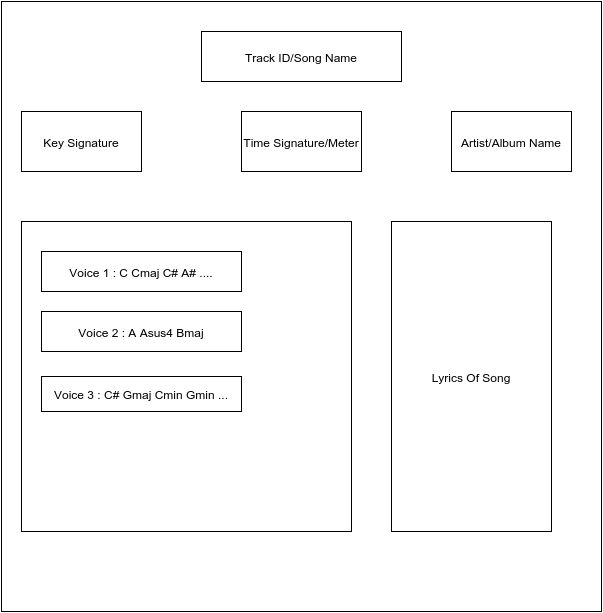
\includegraphics[width=\columnwidth, height=75mm]{DocumentStructureOfModulo7.png}}}
 \caption{Modulo7 internal representation.}
 \label{fig:document}
\end{center}
\end{figure}

\item \textbf{Music theory Models: } Modulo7 implements vector space models derived from \cite{similie} with extensions to polyphonic music and chords using a template matching algorithm described in \cite{chord-detection}. This forms a mathematical formulation of music sources. Its described in detail in section \ref{vecmodels}.

\item \textbf{Client side Querying: } Modulo7 implements client side abstractions that exposes two modes of information retrieval. Both these modes leverage the vector space models defined previously. 
\begin{enumerate}
\item \textbf{Structured Querying: } The structured querying mode allows a user to make SQL like queries based on certain criteria or statistic that is quantified on music theoretic criteria. Its described in section \ref{structuredquery}
\item \textbf{Custom Search Engine: } Modulo7 exposes a search engine functionality but allowing for customized similarity metric choices as described in section \ref{searchengine} 
\end{enumerate}

\item \textbf{Lyrics Engine: } On top of providing support for music sources, Modulo7 also implements a standard text based retrieval model on lyrics of songs written in Apache Lucene. 

\end{enumerate}

\subsection{Consumer Workflow} 

The consumer workflow can be defined as the steps/operations the user takes to initialize the Modulo7 system and output generated on search and structured queries. 

\begin{enumerate}
\item Modulo7 is initialized by specifying a source directory. Every music source file inside the directory is parsed and converted to either an in memory and/or persistent store version. It also indexes these songs on global properties (artist, key-signature, time-signature etc). It also guesstimates certain properties if not explicitly present (e.g key signature via the KK Tonality profiles key finding \cite{kkTonalityKeyFinding} algorithm)
\item It then exposes a prompt which asks the user for two modes (search engine/structured querying). (In either case the appropriate vector space model is built)
\begin{enumerate}
\item If the user selects the search engine functionality, Modulo7 similarity engine then asks for an input query song and a similarity metric (from one of the choices described in section \ref{searchengine}). Then the engine proceeds to rank the query song with each of the indexed songs based on the similarity metric and then returns an ordered list of "relevant" song(based on the similarity scores for each of the indexed songs against the query song). 
\item If the user selects the structured querying mode, Modulo7 asks for an input query along with a set of music theoretic predicates songs must satisfy (details in section \ref{structuredquery}). Any song that satisfies this query is deemed relevant and returned to the user.  
\end{enumerate}
\item Modulo7 optionally caches results in memory so that it does not have to recompute queries.

\end{enumerate}

\section{Vector Space Models for Music Sources} \label{vecmodels}

The vector space models form the core of the search and query functionality of Modulo7. Vector space models are derived from quantification of music theoretical representations of songs and extends functionality of the SIMILIE \cite{similie} melodic similarity library.

\subsection{Building Blocks of unified internal representation}

All vector space models are built from the unified internal representation of songs in Modulo7. 

\begin{enumerate}
\item \textbf{Note:} A note is a pair of pitch(deterministic frequency played by an instrument) and onset (time instance at which a pitch is played). A \textbf{Chord} is a set of pitches played at the same onset. 
\item \textbf{Interval:} The difference between two note pitches.
\item \textbf{Voice:} A set of notes or chords played in succession(usually on a single instrument).
\item \textbf{Song: } A song is a set of interleaved voices, along with some global properties (key signature, time-signature, artist, album etc)
\end{enumerate}

\subsection{Global Vector Space Models} \label{globalvectorspace}

Now once the above building blocks are ascertained for songs, some vector space models can be defined over the entire song. Modulo7 implements 6 such vector space models. Some notable examples are 

\begin{enumerate}
\item \textbf{Normalized Tonal Histogram Vector} : For each of the 12 intervals in western music, compute the frequencies of each and divide by total number of intervals over the song. This forms a 12 dimensional vector irrespective of length of song. Mathematically
\begin{equation}
NTH(S) = <\Delta p^f_1, \Delta p^f_2, ... , \Delta p^f_{12}>
\end{equation}
Here $\Delta p^f_i$ is the fraction of the number of occurrences of the $i^{th}$ interval.
\item \textbf{Normalized Tonal Duration Histogram Vector} : For each of the 12 intervals in western music, compute the cumulative durations each of these intervals are played and divide by total duration of the song. This forms a 12 dimensional vector irrespective of length of song. Mathematically 

\begin{equation}
NTDH(S) = <\Delta t^f_1, \Delta t^f_2, ... , \Delta t^f_{12}>
\end{equation}

Here $\Delta t^f_1$ is the fraction of the duration that the  $i^{th}$ interval is played.  
 
\end{enumerate}

\subsection{Voice specific vector space models} \label{voicespecificvectorspace}
 
Considering each voice as a separate entity, a voice can be modeled as a vector independent of other voices in a song. A particular song can then be represented as a set of these vectors. Some notable examples of these are 

\begin{enumerate}
\item \textbf{Pitch Interval Vector:} If a voice has k pitches played one after the other, there are  k - 1 intervals (for each pitch its immediate subsequent pitch). The pitch interval vector is the chronological succession of these intervals. Mathematically 

\begin{equation}
PI = <\Delta p_1, \Delta p_2, ... , \Delta p_n>
\end{equation}

Here $\Delta p_i$ is the $i^{th}$ interval which is the difference between the $i^{th}$ and $(i - 1)^{th}$ pitches. 

\item \textbf{Rhythmically weighted Pitch Interval Vector:} Similar to the pitch interval vector, except it also takes into account the time $t_i$ an interval $\Delta p_i$ is played for. Mathematically

\begin{equation}
RPI = <rp_1, rp_2, ... , rp_n>
\end{equation}

Here $rp_i$ = $\Delta p_i \times t_i$

\end{enumerate}

\noindent Its important to note that these vectors have a dimensionality influenced by the length of the voices in a song. 
 
\section{Consumer facing abstractions} 

Modulo7 exposes two consumer facing abstractions used to facilitate acquiring relevant songs. 

\subsection{Search Engine Functionality} \label{searchengine}

Based on the vector space models defined in sections \ref{globalvectorspace} and
\ref{voicespecificvectorspace}, customized similarity metrics can be defined to form ranked search functionality for a given query song against an indexed data set. These similarity metrics are derived from the SIMILIE project \cite{similie} and extended ideas in \cite{smithwatermanmusic}. Given two songs $S_1$ and $S_2$, we can define similarity to be 

\begin{equation}
Sim(S_1, S_2) \in \{0, 1\}
\end{equation}

\noindent The definition of $Sim(S_1, S_2)$ can be implemented in various ways and Modulo7 allows the consumer to choose the similarity metric as a custom argument. So for a given query song $S_{query}$ and a given similarity metric Sim, we can define the order list $Or(S_{query}, Sim)$ given the indexed set of songs $S_{ind}$

\begin{equation}
\begin{aligned}
Or(S_{query}, Sim) =  desc\_sort_k \\ \{S | Sim(S_{query}, S) = k, S \in S_{ind}\}
\end{aligned}
\end{equation}

\noindent This order list is presented as an output to the consumer. Modulo7 implements 7 different similarity measures. Following are some notable examples

\begin{enumerate}
\item \textbf{Smith Waterman Song Similarity}: Given two voices $V_1$ and $V_2$, Modulo7 uses the smith waterman genome alignment algorithm \cite{smithwatermanmusic} to estimate similarity based on notes as units. In order to extend this to songs, pair wise voice similarities are calculated and the max similarity is returned. Mathematically 

\begin{equation}
\begin{aligned}
SM(S_1, S_2) = arg_{max} k \{SMV(V_i, V_j) \\ = k | V_i \in S_1, V_j \in S_2)\}
\end{aligned}
\end{equation} 

\item \textbf{N Grams Similarity }: Voices can be defined as N grams (strings of n length n of continuous notes/chords) as defined in \cite{similie}. These n grams can be aggregated over all voices and measures like ukkonnen, count distance and scm trigram (defined in \cite{similietechnicalmanual})
\end{enumerate}

\subsection{Structured Querying Functionality} \label{structuredquery}

\noindent Modulo7 implements a custom SQL like language with its own grammar definition and implementation. Any query can be constructed as 

\begin{equation}
\begin{aligned}
select \ input\_types \ from \\\ DATABASE\_NAME \\ where (boolean\_formula)
\end{aligned}
\end{equation}

Here the individual components stand for 

\begin{enumerate}
\item \textbf{Input Types: } A list of the input types we are interested in. For example if we are only interested in midi files then this value is "midi". If we are interested in more than one type(e.g midi and musicxml) then Input Types = "midi, musicxml". 
\item \textbf{DATABASE\_NAME} : A placeholder for the of the data base (created when Modulo7 server starts up)
\item \textbf{boolean\_function} : A boolean function is a well formed propositional formula (chain of propositions or predicates connected by AND/ORs). Each predicate can either be defined as a criteria or statistic condition.   
\end{enumerate}

\subsection{Criteria}

A criteria is a particular music theoretic condition that a song either satisfies or not. Some notable supported criteria are 

\begin{enumerate}
\item Polyphony criteria : Whether a song is polyphonic or not
\item Key Signature criteria : Whether a song has a particular key signature
\item STAB Voice Criteria : Whether a song follows the Soprano, Alto, Tenor, Bass Voice structures as defined in \cite{satbcriteria}
\end{enumerate}

\subsection{Statistic}

A statistic is a real number generated when applied to a particular song. A statistic condition is defined when this generated statistic satisfies a relational operator with a given thresh-hold value. For example PowerIndex(song) $<$ 0.5 is a valid statistic condition. Some notable supported statistic conditions are 

\begin{enumerate}
\item Average Pitch Duration over the song duration. 
\item Happiness Index : Fraction of major intervals over the total number of intervals
\item Power Index : Fraction of perfect intervals over the total number of intervals
\item Sadness Index : Fraction of minor intervals over the total number of intervals
\end{enumerate}

Given the definition of statistic or criteria (cumulatively called conditions) a boolean formula can be defined as 

\begin{equation}
boolean\_formula = cond_1 \ op_1 \ cond_2 \ .. \ op_{n-1} \ cond_n
\end{equation}
 
\noindent Here $op_i$ is a boolean operator (and/or).  

\section{Experimental Evaluation}

This section includes improvements that have been attained over existing frameworks and input sources. For the purposes of this experiment, existing datasets such as the Saarland dataset \cite{saarlandmsd}, the Wikifonia Dataset \cite{WikifoniaDataset} and the million song data set \cite{msd}. 

\subsection{Indexing and Persistent Store Improvements}

Modulo7 achieves significant storage improvements over the input formats, while not losing any symbolic information. Figure \ref{fig:storageimprovement} illustrates this for the Saarland dataset \cite{saarlandmsd} \\

\begin{figure}[h]
\begin{center}
{\framebox{
 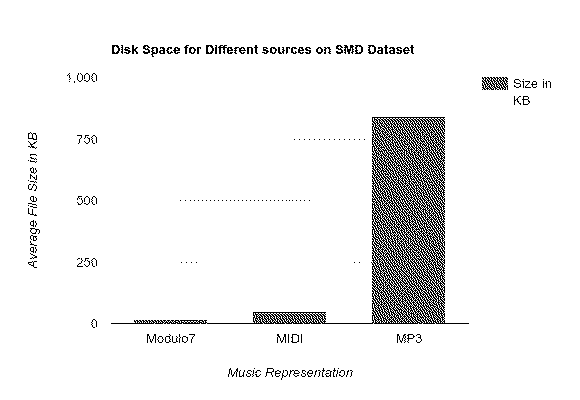
\includegraphics[width=\columnwidth]{BarGraph2.png}}}
 \caption{Space storage improvements over Saarland Dataset.}
 \label{fig:storageimprovement}
\end{center}
\end{figure}

\noindent Similarly an experiment was carried out to ascertain compression as a function of data set size for the Wikifonia Dataset \cite{WikifoniaDataset}

\begin{figure}[h]
\begin{center}
{\framebox{
 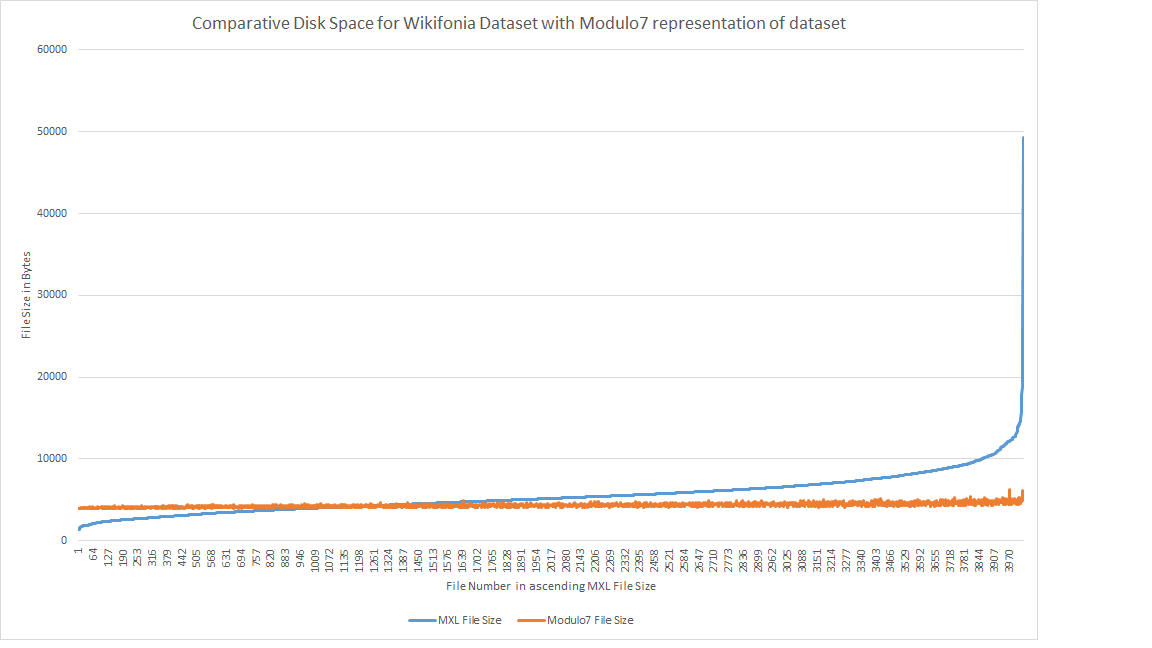
\includegraphics[width=\columnwidth]{M7Graph.png}}}
 \caption{Modulo7 compression of Wikifonia Dataset over increasing subset sizes}
 \label{fig:compression}
\end{center}
\end{figure}

\subsection{Comparisons against JSymbolic}

Some experiments were conducted against the jSymbolic component in the jMIR \cite{jMIR} software suite. Like the jMIR suite, Modulo7 extracts features from songs, but with a different goal (relevance querying and similarity against jMIRs genre classification goals). Modulo7 implements \textbf{23} of jSymbolic's \textbf{111} features. Moreover both frameworks are written in Java and hence language features do not influence the evaluation. \\ 

\noindent The experiment involved comparing memory footprints and time taken for extraction of 23 features for both libraries over increasing subset sizes of the Saarland \cite{saarlandmsd} dataset. 

\begin{figure}[h]
\begin{center}
{\framebox{
 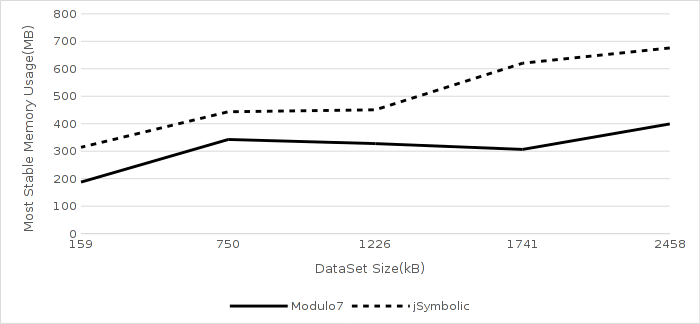
\includegraphics[width=\columnwidth]{MemoryTaken.png}}}
 \caption{Average Memory taken for feature extraction, jSymbolic vs Modulo7}
 \label{fig:MemoryTaken}
\end{center}
\end{figure}

\begin{figure}[h]
\begin{center}
{\framebox{
 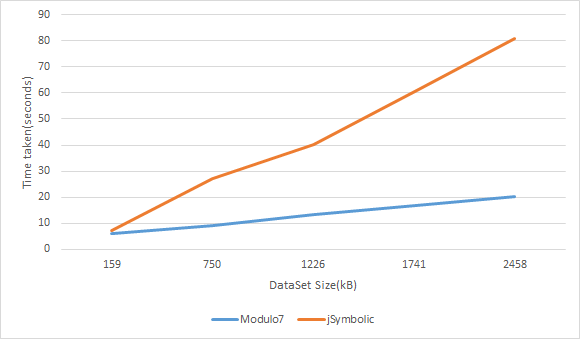
\includegraphics[width=\columnwidth]{TimeTaken.png}}}
 \caption{Total time taken for feature extraction, jSymbolic vs Modulo7}
 \label{fig:TimeTaken}
\end{center}
\end{figure}

\noindent It can be inferred that Modulo7 outperforms jSymbolic in feature extraction and scales better with increasing data set sizes. 

\subsection{Similarity Search Experiments}

\noindent In order to estimate the efficacy of the similarity search algorithms, the million song dataset or MSD \cite{msd} was chosen to act as ground truth. MSD contains tags associated with songs (genre, comments about mood of the song and other such keywords) which was extracted by the researchers using the Last FM API. The ground truth of similarity was based on the number of matching tags between two songs. Consider tag sets $T_i$ and $T_j$ for songs in the MSD $S_i$ and $S_j$. The ground truth similarity is defined as 

\begin{equation} \label{taghitrate}
GTSim(S_1, S_2) = \sum_{t_i \in T(S_1)} \sum_{t_j \in T(S_2)} \begin{cases} 
      1 & t_i == t_j \\
      0 & otherwise \\  \end{cases}
\end{equation}

\noindent The measure was not normalized as MSD had a large number of "junk" tags (irrelevant comments about songs) which would have influenced the ground truth otherwise. \\

\noindent A direct download-able subset of the million song data set was used which contained 10000 songs. A ten fold cross validation was performed (1000 query songs, 9000 data hold out) and average precision and recall are calculated. 

\begin{table}[h]
\begin{center}
    \begin{tabular}{| l | l | l |}
    \hline
    Similarity Measure & Average Recall & Average Precision \\ \hline
    SCM Trigram & 0.308 & 0.299 \\ \hline
    Ukkonnen & 0.339 & 0.291 \\ \hline
    Count Distance & 0.294 & 0.283  \\ \hline
    Tonal Histogram & 0.341 & 0.362  \\ \hline
    \end{tabular}
\end{center}
\caption{Average Precision and Recall for Melodic Similarity Measures}
\end{table}

\subsection{Exploratory Query Search Experiments}

In order to ascertain the effectiveness of the query engine, certain custom experiments were ran. Queries built from concepts 

\begin{table}[!htb]
\begin{center}
    \begin{tabular}{| l | l | l | l |}
    \hline
    Purpose &  Query & Precision  & Recall \\ \hline
    Rock Song ID &  Q1 & 0.13  & 0.98 \\ \hline
    Sad Song ID &  Q2 & 0.02  & 0.44 \\ \hline
    Happy Song ID &  Q3 & 0.018  & 0.4 \\
    \hline
    \end{tabular}
\end{center}
\caption{Results for the exploratory query analysis}
\end{table}

\noindent We define Q1, Q2 and Q3 as follows

\begin{enumerate}
\item [Q1] select mp3 from default\_database where powerindex $>$ 0.61; with a ground truth estimate as song tags being either "rock" or "pop\_rock"
\item [Q2] select mp3 from default\_database where sadnessindex $>$ 0.15 and scale = minor; with the ground truth estimate being song tags either "sad" or "sad\_songs" 
\item [Q3] select mp3 from default\_database where happinessindex $>$ 0.11 and scale = major; with ground truth being song tags as either "happy" or "happy\_song"s
\end{enumerate}





\section{Conclusion and Future Work}


% For bibtex users:
\bibliography{ISMIRtemplate}

\end{document}
